% Provenance (never printed): old premiere S material on plate kinematics (rigid
% plates, rates from magnetic anomalies and from satellite positioning, hotspots
% and the Hawaiian chain, the coherence of the model); see
% sources/book2/PROVENANCE.md. Velocities from the NNR-MORVEL56 poles
% (figdata/grade-11/plate_velocities.py), station series from the Nevada Geodetic
% Laboratory (gnss_series.py), volcano ages from Clague and Dalrymple 1987
% (hawaii_chain.py). Euler poles and triple junctions belong to Year 1: the
% rotation pole is told, not defined.
\chapter{Platen en hun bewegingen}\label{ch:g11:plate-motions}

Vlak bij de top van de Mauna Kea, op het eiland Hawaii, staat een antenne die aan
het gesteente is vastgezet en die sinds oktober 1996 elke dag de signalen van
plaatsbepalingssatellieten ontvangt. Elke dag berekent een computer waar de
antenne staat, tot op een paar millimeter. Dertig jaar aan posities vertellen elk
jaar hetzelfde verhaal: de antenne, de berg en het hele eiland bewegen ongeveer
\qty{7}{cm} per jaar naar het west-noordwesten, zonder te stoppen en zonder te
draaien. In 2026 stond de antenne meer dan twee meter van haar beginpunt. Dit
hoofdstuk meet zulke bewegingen, laat zien hoe ze op een bol in elkaar passen, en
leest dezelfde beweging af in de keten van dode vulkanen die zich van Hawaii
door het noorden van de Grote Oceaan uitstrekt.
% ledger: data:b2-ngl-gnss

\begin{recall}
De \omterm{def:g11:lithosphere-asthenosphere:lithosphere}{lithosfeer} is gebroken in tektonische platen die ten opzichte van elkaar
bewegen met een paar centimeter per jaar; hun grenzen zijn ruggen, troggen,
botsingszones en transformbreuken (Boek 1, jaar 7). Een hotspot is een plaats
diep in de mantel die een vulkaan voedt op de plaat erboven; de plaat voert de
vulkaan mee terwijl er boven de hotspot een nieuwe groeit (Boek 1,
jaar 7). Een ontvanger voor satellietplaatsbepaling berekent zijn eigen positie
uit de signalen van verscheidene satellieten (Boek 1, jaar 9). De magnetische strepen
van de oceaanbodem geven de \omterm{def:g11:drift-to-spreading:spreading-rate}{spreidingssnelheid} van een rug
(\cref{ch:g11:drift-to-spreading}), en de \omterm{def:g11:lithosphere-asthenosphere:lithosphere}{lithosfeer} is de starre buitenste
schil van de Aarde, ongeveer \qty{100}{km} dik
(\cref{ch:g11:lithosphere-asthenosphere}). Een snelheid van \qty{1}{cm} per jaar is
\qty{10}{km} per miljoen jaar, en \qty{1}{mm} per jaar is \qty{1}{km} per
miljoen jaar.
\end{recall}

\begin{omfigure}
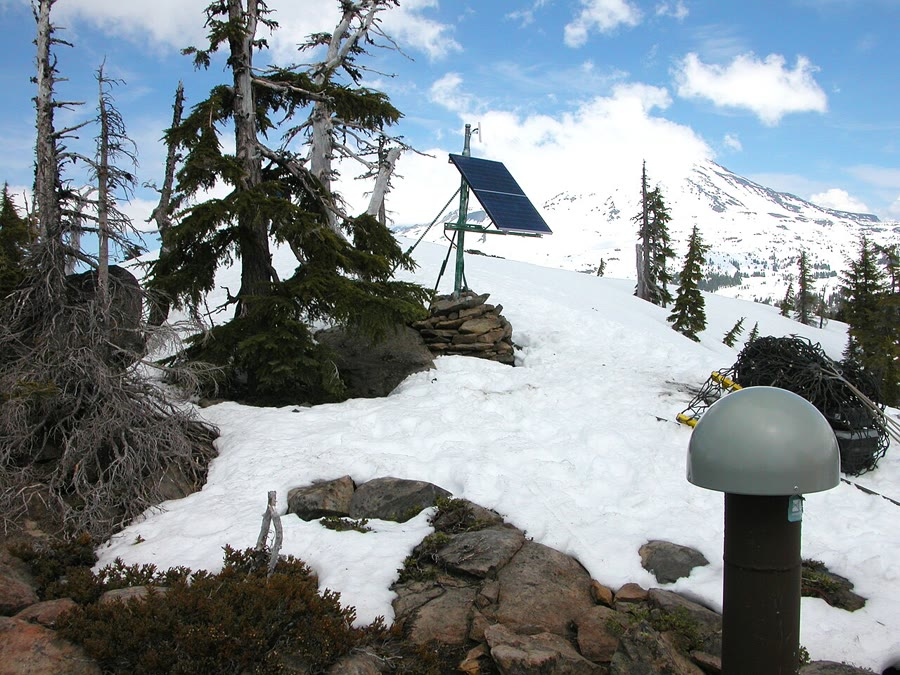
\includegraphics[width=0.62\linewidth]{images/book2/g11-usgs-gps-station.jpg}

{\small Een vast station voor satellietplaatsbepaling op een vulkaan in de
Cascade Range, Oregon (2007). De antenne zit onder de grijze koepel, op een mast
die stevig in de grond staat; het zonnepaneel erachter voedt de ontvanger. Zo'n
station registreert dag na dag zijn eigen positie. Foto: Dave Sherrod,
USGS (publiek domein).}
\end{omfigure}
% ledger: photo:g11-gps-station

\section{Starre platen op een bol}

Aardbevingen liggen niet willekeurig over de Aarde verspreid: bijna allemaal
vinden ze plaats langs smalle gordels, de plaatgrenzen (Boek 1, jaar 7). Binnen een
plaat breekt het gesteente nauwelijks. Een plaat is dus geen zacht vel dat
uitrekt en rimpelt terwijl het beweegt, maar een stijf stuk \omterm{def:g11:lithosphere-asthenosphere:lithosphere}{lithosfeer} dat
als geheel beweegt.

\begin{definition}[Starre plaat]\label{def:g11:plate-motions:rigid-plate}
Een \emph{starre plaat}\index{starre plaat} is een stuk \omterm{def:g11:lithosphere-asthenosphere:lithosphere}{lithosfeer} dat als één
blok beweegt: de afstanden tussen punten erop veranderen niet, en de vervorming
is samengebracht in smalle zones langs de grenzen.
\end{definition}

Het model van starre platen is een benadering. Sommige gebieden vervormen over
honderden kilometers, zoals de hoogvlakten achter de Himalaya of het westen van
Noord-Amerika, en het model behandelt ze als brede grenzen. Maar over het grootste
deel van het aardoppervlak werkt het opmerkelijk goed: de snelheden die het voor
starre platen voorspelt, komen tot op een paar millimeter per jaar overeen met wat
satellietstations meten (\cref{sec:g11:plate-motions:predictive}), terwijl platen
met centimeters per jaar ten opzichte van elkaar bewegen.

Hoe kan een starre kap over het oppervlak van een bol bewegen? Ze kan niet in een
rechte lijn glijden, want een rechte lijn verlaat de bol. Wat de beweging van een
starre kap ook is, het is een \emph{rotatie} om een as door het middelpunt van de
Aarde. De as snijdt het oppervlak in de \emph{rotatiepool} van de plaat. Een
punt op de plaat beweegt langs een kleine cirkel rond die pool, en hoe
verder het van de pool ligt, hoe groter zijn cirkel en hoe sneller het beweegt
(figuur hieronder). Het bewijs dat elke beweging van een
starre kap zo'n rotatie is, en het gebruik van rotatiepolen om plaatgrenzen te
beschrijven, horen bij Boek~3; hier worden alleen de snelheden gebruikt.

\begin{omfigure}
\begin{tikzpicture}[scale=1.15, font=\footnotesize]
  \fill[omSea!45] (0,0) circle (2);
  \draw (0,0) circle (2);
  % small circles about the rotation pole (pole at the top), seen slightly from above
  \foreach \a/\len in {60/0.75, 35/1.23, 0/1.5} {
    \pgfmathsetmacro{\r}{2*cos(\a)}
    \pgfmathsetmacro{\h}{2*sin(\a)}
    \draw[black!45, densely dashed] (-\r,\h) arc[start angle=180, end angle=0, x radius=\r, y radius=0.22*\r];
    \draw[omDef!80!black, line width=0.7pt] (-\r,\h) arc[start angle=180, end angle=360, x radius=\r, y radius=0.22*\r];
    \draw[-{Stealth[length=5pt]}, omProp, line width=1.1pt] (0,\h-0.22*\r) -- ++(\len,0);
  }
  \draw[black!70, dash pattern=on 3pt off 2pt] (0,-2.5) -- (0,2.55);
  \fill (0,2) circle (1.6pt);
  \node[anchor=south west] at (0.05,2.02) {rotatiepool};
  \node[anchor=north, text=black!70] at (0,-2.5) {rotatieas, door het middelpunt};
  \fill (0,0) circle (1pt);
  \node[anchor=west, align=left] at (2.25,0.9) {elk punt beweegt\\langs een kleine cirkel\\rond de pool};
  \node[anchor=west, align=left, text=omProp] at (2.25,-0.4) {snelheid: het grootst\\\ang{90} van de pool};
\end{tikzpicture}

{\small Een \omterm{def:g11:plate-motions:rigid-plate}{starre plaat} op een bol draait om een as door het middelpunt van
de Aarde. Punten dicht bij de rotatiepool bewegen langzaam, langs kleine cirkels;
punten op \ang{90} van de pool bewegen het snelst (pijlen: snelheden op schaal).}
\end{omfigure}

De snelheid van een punt is makkelijk te berekenen. Een punt op een hoekafstand
$\theta$ van de pool ligt op de afstand $R\sin\theta$ van de as, waarbij
$R = \qty{6371}{km}$ de straal van de Aarde is. Als de plaat $\omega$
graden per miljoen jaar draait, legt het punt in een miljoen jaar het deel
$\omega/360$ af van de cirkel met straal $R\sin\theta$:
\[
  v = \frac{\omega}{360} \times 2\pi R\sin\theta
    = \frac{\pi\,\omega}{180}\,R\sin\theta .
\]
Voor $\omega = \qty{1}{\degree}$ per miljoen jaar en $\theta = \ang{90}$
is dat $\pi \times 6371/180 \approx \qty{111}{km}$ per miljoen jaar,
\qty{11.1}{cm} per jaar. Een plaat heeft dus geen enkelvoudige snelheid: haar punten
bewegen met snelheden van nul bij de rotatiepool (als de pool op de
plaat ligt) tot een maximum op \ang{90} ervan. De transformbreuken langs een rug,
waarlangs twee platen langs elkaar glijden, lopen langs kleine cirkels rond de
pool van de relatieve rotatie van de twee platen.
% ledger: earth:Rmean (shared), nnr56:poles

Gepubliceerde reeksen rotatiepolen geven voor elke plaat de positie van haar
pool en haar draaisnelheid. Een ervan, vooral opgebouwd uit de spreidingssnelheden
en de spreidingsrichtingen die langs de ruggen zijn gemeten, beschrijft 56
platen; de Pacifische plaat draait met
\ang{0.651} per miljoen jaar, de Euraziatische plaat met \ang{0.223}. Uit deze
getallen berekent een computer de snelheid van elk punt van elke plaat
(kaart hieronder).
% ledger: nnr56:poles, nnr56:data

\begin{omfigure}
\begin{tikzpicture}
\begin{axis}[ommap, width=\linewidth, xtick={-180,-90,...,180}, ytick={-60,0,60}]
\addplot[fill=omLithAlluv, draw=black!45, line width=0.2pt] table {figdata/out/shared-geo-land.dat};
\addplot[omRidge, line width=0.6pt] table {figdata/out/shared-geo-school-ridge.dat};
\addplot[omRidge!70!black, line width=0.6pt] table {figdata/out/shared-geo-school-transform.dat};
\addplot[omTrench, line width=0.6pt] table {figdata/out/shared-geo-school-subduction.dat};
\addplot[fill=omTrench, draw=none] table {figdata/out/shared-geo-school-teeth.dat};
\addplot[black!65, line width=0.6pt] table {figdata/out/shared-geo-school-collision.dat};
% computed in figdata/grade-11/plate_velocities.py (NNR-MORVEL56); 2.5 degrees per cm/yr
\addplot[black, line width=0.8pt, -{Stealth[length=4pt]}, quiver={u=\thisrow{dx}, v=\thisrow{dy}}]
  table[x=lon, y=lat] {figdata/out/grade-11-plate_velocities-arrows.dat};
\addplot[omProp, line width=1.2pt, -{Stealth[length=5pt]}, quiver={u=\thisrow{dx}, v=\thisrow{dy}}]
  table[x=lon, y=lat] {figdata/out/grade-11-plate_velocities-hawaii.dat};
\addplot[only marks, mark=*, mark size=1.3pt, omProp] coordinates {(-155.46,19.80)};
\node[font=\scriptsize, anchor=north, fill=white, fill opacity=0.75, text opacity=1, inner sep=1pt]
  at (axis cs:-150,15) {Mauna Kea};
\draw[black, line width=0.8pt, -{Stealth[length=4pt]}] (axis cs:-172,-80) -- (axis cs:-147,-80);
\node[font=\scriptsize, anchor=west, fill=white, fill opacity=0.75, text opacity=1, inner sep=1pt]
  at (axis cs:-145,-80) {\qty{10}{cm} per jaar};
\end{axis}
\end{tikzpicture}

{\small De snelheden van punten binnen 16 platen, berekend uit hun
gepubliceerde rotatiepolen, in een referentiestelsel waarin de \omterm{def:g11:lithosphere-asthenosphere:lithosphere}{lithosfeer} als
geheel niet draait. De Pacifische, Nazca-, Cocos-, Australische en Indische plaat
bewegen het snelst; de Euraziatische, Noord- en Zuid-Amerikaanse en Antarctische
plaat langzaam. Rode pijl: de Pacifische plaat bij de Mauna Kea. Rotatiepolen:
Argus, Gordon en DeMets (2011); plaatgrenzen: Bird (2003); land: Natural Earth.}
\end{omfigure}
% ledger: nnr56:poles, data:pb2002, data:ne-land

\section{De bewegingen meten}

\subsection{Twee manieren om een snelheid te meten}

De magnetische strepen van de oceaanbodem geven de snelheid waarmee twee platen
over een rug uit elkaar bewegen (\cref{ch:g11:drift-to-spreading}): deel de
afstand van een streep tot de as van de rug door haar ouderdom. De verkregen
snelheid is een gemiddelde over de ouderdom van de streep, vaak de laatste paar
miljoen jaar, en het is een \emph{relatieve} snelheid, die van de ene plaat gezien
vanaf de andere. Strepen zeggen niets over platen die elkaar ontmoeten bij een
trog of een botsingszone, want daar wordt geen oceaanbodem gemaakt.

Satellietplaatsbepaling meet de beweging van één enkel punt, vandaag, over een
paar jaar of decennia. Een vast station is aan vast gesteente verankerd, zodat
het met de plaat meebeweegt; zijn dagelijkse posities, uitgezet tegen de tijd,
liggen op een rechte lijn waarvan de helling de snelheid van het station is.

\begin{method}[Een snelheid uit een tijdreeks van posities]\label{met:g11:plate-motions:rate}
\begin{enumerate}
  \item Zet de oostpositie en de noordpositie van het station uit tegen de
        tijd, in twee grafieken of in dezelfde grafiek.
  \item Trek de rechte lijn die elke reeks het best volgt (of lees er twee
        punten ver uit elkaar op af). Haar helling, in millimeter per jaar, is de
        oostsnelheid $v_E$ of de noordsnelheid $v_N$; een station dat naar het
        westen of zuiden beweegt, heeft een negatieve snelheid.
  \item De snelheid van het station is $v = \sqrt{v_E^2 + v_N^2}$; haar richting
        maakt met de oost-westlijn de hoek $\alpha$ zodat
        $\tan\alpha = |v_N|/|v_E|$, naar het noorden als $v_N > 0$ en naar
        het oosten als $v_E > 0$.
\end{enumerate}
\end{method}

\begin{omfigure}
\begin{tikzpicture}
\begin{axis}[ompt, name=a, width=0.5\linewidth, height=5.6cm, xmin=1995, xmax=2027, ymin=-200, ymax=120,
  xlabel={jaar}, ylabel={positie (\unit{cm})}, xtick={2000,2010,2020},
  xticklabel style={/pgf/number format/set thousands separator={}},
  title={\small Mauna Kea, Hawaii (MKEA)}, tick label style={font=\scriptsize}]
% computed in figdata/grade-11/gnss_series.py; ledger: data:b2-ngl-gnss
\addplot[only marks, mark=*, mark size=0.5pt, omDef] table[x=year, y=north] {figdata/out/grade-11-gnss_series-mkea.dat};
\addplot[only marks, mark=*, mark size=0.5pt, omProp] table[x=year, y=east] {figdata/out/grade-11-gnss_series-mkea.dat};
\node[font=\scriptsize, text=omDef!80!black, anchor=west] at (axis cs:1996.5,80) {noord};
\node[font=\scriptsize, text=omProp!80!black, anchor=west] at (axis cs:1996.5,-120) {oost};
\end{axis}
\begin{axis}[ompt, at={(a.east)}, anchor=west, xshift=0.9cm, width=0.5\linewidth, height=5.6cm, xmin=1995, xmax=2027,
  ymin=-10, ymax=70, xlabel={jaar}, xtick={2000,2010,2020},
  xticklabel style={/pgf/number format/set thousands separator={}},
  title={\small Wettzell, Duitsland (WTZR)}, tick label style={font=\scriptsize}]
\addplot[only marks, mark=*, mark size=0.5pt, omDef] table[x=year, y=north] {figdata/out/grade-11-gnss_series-wtzr.dat};
\addplot[only marks, mark=*, mark size=0.5pt, omProp] table[x=year, y=east] {figdata/out/grade-11-gnss_series-wtzr.dat};
\node[font=\scriptsize, text=omDef!80!black, anchor=west] at (axis cs:2014,22) {noord};
\node[font=\scriptsize, text=omProp!80!black, anchor=west] at (axis cs:2006,40) {oost};
\end{axis}
\end{tikzpicture}

{\small Maandgemiddelde posities van twee vaste stations, gemeten vanaf hun
eerste maand: oost (rood) en noord (blauw). Elke reeks ligt op een
rechte lijn, waarvan de helling de snelheid van het station in die richting is. De Mauna Kea, op de Pacifische plaat, beweegt naar het westen en noorden; Wettzell, op
de Euraziatische plaat, naar het oosten en noorden, ongeveer drie keer zo langzaam. Gegevens:
Nevada Geodetic Laboratory (Blewitt, Hammond en Kreemer, 2018).}
\end{omfigure}
% ledger: data:b2-ngl-gnss

\begin{example}[Het station op de Mauna Kea]\label{ex:g11:plate-motions:mkea}
Van oktober 1996 tot september 2026 volgen de maandelijkse posities van het
station op de Mauna Kea twee rechte lijnen met hellingen $v_E =
\qty{-63.2}{mm}$ per jaar (naar het westen) en $v_N = \qty{+34.5}{mm}$ per jaar. De
snelheid is $\sqrt{63.2^2 + 34.5^2} \approx \qty{72}{mm}$ per jaar, en $\tan\alpha
= 34.5/63.2 \approx 0.546$ geeft $\alpha \approx \ang{29}$: het station beweegt
\qty{7.2}{cm} per jaar in een richting \ang{29} ten noorden van het westen. De
rotatiepool van de Pacifische plaat voorspelt op deze plaats \qty{6.9}{cm} per jaar,
\ang{28} ten noorden van het westen.
\end{example}
% ledger: data:b2-ngl-gnss, nnr56:poles (prediction computed in plate_velocities.py)

De punten liggen een paar millimeter rond de lijnen verspreid, veel minder dan de
beweging van één jaar: na een paar jaar meten is de snelheid van een station
beter dan tot op een millimeter per jaar bekend.

\subsection{Relatieve en absolute beweging}

Een snelheid wordt altijd gemeten ten opzichte van iets. Het station op de Mauna
Kea beweegt \qty{7.2}{cm} per jaar ten opzichte van een referentiestelsel dat aan
de hele Aarde vastzit; gezien vanaf een station in Noord-Amerika, dat zelf beweegt,
is zijn snelheid anders.

\begin{definition}[Relatieve beweging; absolute beweging]\label{def:g11:plate-motions:relative-motion}
De \emph{relatieve beweging}\index{relatieve beweging} van een plaat $A$ ten
opzichte van een plaat $B$ is haar beweging zoals een waarnemer die op $B$ staat
die ziet. De \emph{absolute beweging}\index{absolute beweging} van een plaat is
haar beweging ten opzichte van een referentiestelsel dat aan de diepe Aarde
vastzit, bijvoorbeeld een reeks hotspots die vast worden verondersteld, of het
stelsel waarin de \omterm{def:g11:lithosphere-asthenosphere:lithosphere}{lithosfeer} als geheel niet draait.
\end{definition}

Ruggen, troggen en transformbreuken worden gevormd door \omterm{def:g11:plate-motions:relative-motion}{relatieve bewegingen}: wat
bij een grens telt, is hoe de twee platen ten opzichte van elkaar bewegen.
Relatieve snelheden worden opgeteld zoals de verplaatsingen die ze veroorzaken.

\begin{proposition}[Relatieve snelheden tellen op als pijlen]\label{prop:g11:plate-motions:sum}
Zij $\vec v_{A/B}$ de snelheid van plaat $A$ ten opzichte van plaat $B$, in een
gegeven punt van de grens, en evenzo voor de andere paren. Voor elke drie
platen $A$, $B$, $C$ geldt
\[
  \vec v_{A/C} = \vec v_{A/B} + \vec v_{B/C},
  \qquad\text{en}\qquad
  \vec v_{B/A} = -\vec v_{A/B}.
\]
\end{proposition}

\begin{proof}
Laat in een korte tijd $\Delta t$ een punt dat aan $A$ vastzit van positie $P$
naar $P'$ gaan, gezien vanaf $C$, en laat het punt van $B$ dat in $P$ was naar
$Q$ gaan, gezien vanaf $C$. Gezien vanaf $B$ is het punt van $A$ van $Q$ naar
$P'$ gegaan. De verplaatsingen tellen op als vectoren:
$\overrightarrow{PP'} = \overrightarrow{PQ} + \overrightarrow{QP'}$, dat wil zeggen:
verplaatsing van $A$ gezien vanaf $C$ = verplaatsing van $B$ gezien vanaf $C$ +
verplaatsing van $A$ gezien vanaf $B$. Delen door $\Delta t$ geeft $\vec v_{A/C}
= \vec v_{B/C} + \vec v_{A/B}$. Met $C = A$ is het linkerlid nul: $\vec
v_{B/A} = -\vec v_{A/B}$.
\end{proof}

\begin{method}[Een snelheidsdriehoek sluiten]\label{met:g11:plate-motions:triangle}
\begin{enumerate}
  \item Schrijf elke bekende snelheid met haar oost- en noordcomponent, allemaal
        in hetzelfde punt gemeten.
  \item Om $\vec v_{A/B}$ te vinden uit de snelheden van $A$ en $B$ in hetzelfde
        stelsel $C$, trek je af: $\vec v_{A/B} = \vec v_{A/C} - \vec v_{B/C}$,
        component voor component.
  \item Zet in een tekening de staarten van $\vec v_{A/C}$ en $\vec v_{B/C}$ in
        hetzelfde punt: de pijl van de punt van $\vec v_{B/C}$ naar de punt van
        $\vec v_{A/C}$ is $\vec v_{A/B}$, en die sluit de driehoek.
  \item Bereken haar lengte en richting zoals in
        \cref{met:g11:plate-motions:rate}.
\end{enumerate}
\end{method}

\begin{example}[De San Andreasbreuk]\label{ex:g11:plate-motions:san-andreas}
In het midden van Californië, op \ang{35.5} NB en \ang{120.5} WL, geven de
rotatiepolen de Pacifische plaat de snelheid $(-42.1, +26.4)$ en de
Noord-Amerikaanse plaat $(-11.9, -14.8)$, in millimeter per jaar (oost, noord), in
het stelsel van de hele \omterm{def:g11:lithosphere-asthenosphere:lithosphere}{lithosfeer}. De Pacifische plaat ten opzichte van Noord-Amerika
beweegt met $(-42.1 + 11.9,\ 26.4 + 14.8) = (-30.2, +41.2)$, dat wil zeggen
$\sqrt{30.2^2 + 41.2^2} \approx \qty{51}{mm}$ per jaar, in een richting
\ang{36} ten westen van het noorden (figuur hieronder). De San
Andreasbreuk, die naar het noordwesten loopt, neemt het grootste deel van dit glijden op.
\end{example}
% ledger: nnr56:poles (computed in plate_velocities.py: relative pa/na at 120.5 W 35.5 N)

\begin{omfigure}
\begin{tikzpicture}[x=0.065cm, y=0.065cm, font=\footnotesize]
  % mm/yr, from plate_velocities.py: PA (-42.1, 26.4), NA (-11.9, -14.8), PA/NA (-30.2, 41.2)
  \draw[black!25] (-8,0) -- (8,0) (0,-8) -- (0,8);
  \draw[-{Stealth[length=5pt]}, omProp, line width=1.1pt] (0,0) -- (-42.1,26.4)
    node[pos=0.55, above right, inner sep=1pt] {$\vec v_{\mathrm{PA}}$};
  \draw[-{Stealth[length=5pt]}, omDef, line width=1.1pt] (0,0) -- (-11.9,-14.8)
    node[pos=0.8, right=2pt] {$\vec v_{\mathrm{NA}}$};
  \draw[-{Stealth[length=5pt]}, black, line width=1.1pt] (-11.9,-14.8) -- (-42.1,26.4)
    node[pos=0.4, left=9pt, align=right] {$\vec v_{\mathrm{PA/NA}}$\\\qty{51}{mm} per jaar};
  \fill (0,0) circle (0.9pt);
  % compass
  \draw[-{Stealth[length=4pt]}] (25,10) -- (25,24) node[above] {N};
  \draw[-{Stealth[length=4pt]}] (25,10) -- (39,10) node[right] {O};
  \draw (25,-18) -- (40.4,-18);
  \node[below] at (32.7,-18) {\qty{20}{mm} per jaar};
  \draw (25,-17) -- (25,-19) (40.4,-17) -- (40.4,-19);
\end{tikzpicture}

{\small Een snelheidsdriehoek sluiten in het midden van Californië (op schaal). Rood:
de Pacifische plaat; blauw: de Noord-Amerikaanse plaat, beide in het stelsel van de
hele \omterm{def:g11:lithosphere-asthenosphere:lithosphere}{lithosfeer}. Zwart: de Pacifische plaat gezien vanaf Noord-Amerika, de
pijl van de punt van de blauwe naar de punt van de rode.}
\end{omfigure}

\section{Hotspotsporen}

\subsection{Een plaat boven een vaste pluim}

Hawaii ligt midden op de Pacifische plaat, meer dan \qty{3000}{km}
van de dichtstbijzijnde plaatgrens.
% ledger: usgs:hawaii-hotspot (Book 1 row)
 Zijn vulkanen worden gevoed door een hotspot (Boek~1,
jaar~7). De plaat beweegt eroverheen, en elke vulkaan wordt van de
hotspot weggevoerd terwijl er achter hem een nieuwe groeit.

\begin{definition}[Hotspotspoor]\label{def:g11:plate-motions:hotspot-track}
Een \emph{hotspotspoor}\index{hotspotspoor} is de rij vulkanen, en
verdronken vulkanen die onderzeese bergen heten, die een plaat van een
hotspot wegvoert terwijl ze eroverheen beweegt: de actieve vulkaan staat boven de
hotspot, en de vulkanen zijn steeds ouder naarmate ze verder ervan liggen.
\end{definition}

\begin{omfigure}
\begin{tikzpicture}[font=\footnotesize]
  % plate moving to the left over a fixed plume (not to scale)
  \fill[omSea!50] (0,0) rectangle (11,0.9);
  \fill[black!22] (0,-0.9) rectangle (11,0);
  \draw (0,0) -- (11,0);
  \draw[densely dashed] (0,0.9) -- (11,0.9) node[right] {zeeniveau};
  \node[anchor=east] at (10.95,-0.45) {lithosfeer};
  \fill[omLithPeridotite!40] (0,-2.3) rectangle (11,-0.9);
  \node[anchor=west] at (0.1,-1.6) {asthenosfeer};
  % plume
  \fill[omProp!55] (8.6,-2.3) -- (8.6,-1.2) .. controls (8.6,-0.9) and (9.2,-0.9) .. (9.2,-1.2) -- (9.2,-2.3) -- cycle;
  \fill[omProp!55] (8.75,-0.95) rectangle (9.05,0);
  \node[anchor=north, align=center] at (8.9,-2.35) {pluim, vast in de mantel};
  % volcanoes: active over the plume, older ones carried left, eroded and sunk
  \fill[black!65] (8.0,0) -- (8.9,1.6) -- (9.8,0) -- cycle;
  \fill[black!55] (5.4,0) -- (6.2,1.15) -- (7.0,0) -- cycle;
  \fill[black!50] (3.0,0) -- (3.55,0.62) -- (3.85,0.62) -- (4.4,0) -- cycle;
  \fill[black!45] (0.8,0) -- (1.25,0.42) -- (1.65,0.42) -- (2.1,0) -- cycle;
  \node[above] at (8.9,1.6) {actief};
  \node[above] at (6.2,1.15) {$t_1$};
  \node[above] at (3.7,0.62) {$t_2$};
  \node[above] at (1.45,0.42) {$t_3$};
  % plate motion
  \draw[-{Stealth[length=6pt]}, line width=1.2pt] (6.5,-0.45) -- (4.0,-0.45) node[left] {plaat beweegt, snelheid $v$};
  % distance d = v t
  \draw[{Stealth[length=4pt]}-{Stealth[length=4pt]}] (3.7,2.3) -- (8.9,2.3) node[midway, above] {$d_2 = v\,t_2$};
  \draw[black!50] (3.7,1.05) -- (3.7,2.4) (8.9,2.0) -- (8.9,2.4);
\end{tikzpicture}

{\small Een plaat die met de snelheid $v$ beweegt boven een pluim die vast in de
mantel zit (niet op schaal). Een vulkaan met ouderdom $t$, gebouwd boven de pluim,
is over de afstand $d = v\,t$ meegevoerd; de oudere vulkanen eroderen en zakken
onder de zeespiegel.}
\end{omfigure}

\begin{proposition}[Snelheid uit een hotspotspoor]\label{prop:g11:plate-motions:hotspot}
Als een hotspot vast blijft in de diepe mantel en de plaat erboven met een
constante snelheid $v$ in een constante richting beweegt, ligt een vulkaan die
een tijd $t$ geleden boven de hotspot stond, nu op de afstand
\[
  d = v\,t
\]
van de actieve vulkaan, langs het spoor. De ouderdommen van de vulkanen, uitgezet
tegen hun afstanden, liggen op een rechte lijn door de oorsprong met
helling $1/v$, en $v$ is de absolute snelheid van de plaat.
\end{proposition}

\begin{proof}
De vulkaan is gebouwd waar de plaat boven de hotspot stond, en is sindsdien met
de plaat meebewogen. Gedurende de tijd $t$ is de plaat over
$v\,t$ in een vaste richting bewogen, dus de vulkaan ligt op die afstand van het
punt van de plaat dat nu boven de hotspot ligt, waar de actieve vulkaan staat. Het
verband $t = d/v$ is dat van een rechte lijn door de oorsprong met helling
$1/v$. De snelheid is gemeten ten opzichte van de hotspot, dat wil zeggen ten
opzichte van de diepe mantel: het is een absolute snelheid.
\end{proof}

\subsection{De Hawaii-Keizerketen}

Vanaf het eiland Hawaii loopt een rij eilanden, riffen en onderzeese bergen zo'n
\qty{3400}{km} naar het west-noordwesten, maakt dan een scherpe bocht en loopt
verder naar het noorden als de Keizerbergen, waarvan de berg Suiko alleen al
\qty{4860}{km} van de Kilauea ligt, tot aan de troggen voor Kamtsjatka en de
Aleoeten (beeld hieronder).
% ledger: cd87:ages

\begin{omfigure}
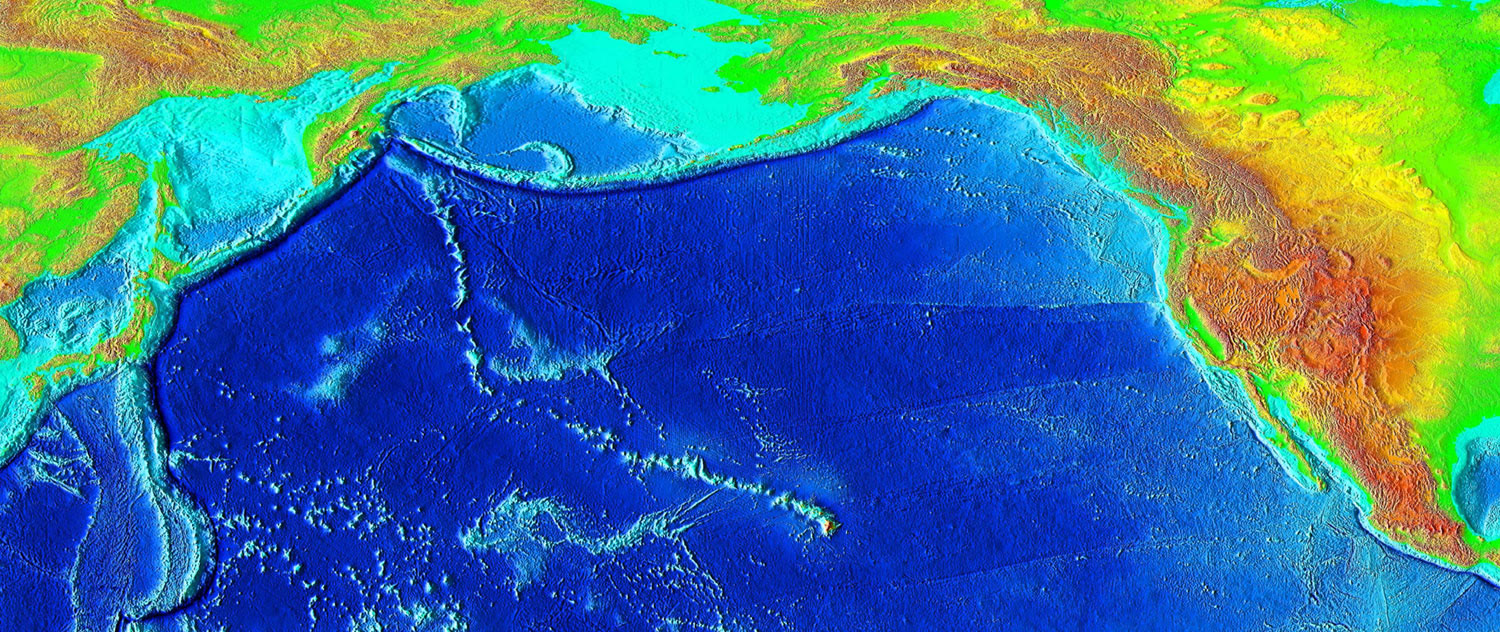
\includegraphics[width=\linewidth]{images/book2/g11-ngdc-hawaii-chain.jpg}

{\small Reliëf van de bodem van het noorden van de Grote Oceaan. De Hawaiiketen
loopt vanaf het eiland Hawaii (onderaan in het midden, bruin) naar het
west-noordwesten; bij de knik buigt ze naar het noorden af in de Keizerbergen, die
eindigen bij de trog langs Kamtsjatka en de Aleoeten. Beeld: National
Geophysical Data Center, NOAA (publiek domein).}
\end{omfigure}
% ledger: photo:g11-hawaii-chain

Kalium-argondatering van lava's van 37 vulkanen van de keten, verzameld op
de eilanden, opgebaggerd van de onderzeese bergen of door hun sedimenten heen
geboord, geeft hun ouderdom (grafiek hieronder). De Mauna Kea is ongeveer
\num{0.4} miljoen jaar oud, Kauai \num{5.1}, Midway \num{27.7}, en de
berg Suiko, bij het verre einde van de Keizerketen, \num{64.7}. De ouderdommen
nemen toe met de afstand tot de Kilauea, de actieve vulkaan, zoals een \omterm{def:g11:plate-motions:hotspot-track}{hotspotspoor}
voorspelt.
% ledger: cd87:ages

\begin{omfigure}
\begin{tikzpicture}
\begin{axis}[ompt, width=0.82\linewidth, height=6.4cm, xmin=0, xmax=5000, ymin=0, ymax=70,
  xlabel={afstand tot de Kilauea langs de keten (\unit{km})}, ylabel={ouderdom (miljoen jaar)},
  xticklabel style={/pgf/number format/set thousands separator={}},
  legend style={font=\scriptsize, at={(0.03,0.97)}, anchor=north west}, legend cell align=left]
% computed in figdata/grade-11/hawaii_chain.py; ledger: cd87:ages
\addplot[only marks, mark=o, mark size=1.6pt, omDef, error bars/.cd, y dir=both, y explicit]
  table[x=dist, y=age, y error=err] {figdata/out/grade-11-hawaii_chain-hawaiian.dat};
\addplot[only marks, mark=triangle, mark size=2pt, omProp, error bars/.cd, y dir=both, y explicit]
  table[x=dist, y=age, y error=err] {figdata/out/grade-11-hawaii_chain-emperor.dat};
\addplot[black, densely dashed, line width=0.6pt] table[x=dist, y=age] {figdata/out/grade-11-hawaii_chain-fit.dat};
\legend{Hawaiiketen, knik en Keizerketen, {lijn door de oorsprong, \qty{9.1}{cm} per jaar}}
\draw[black!50, densely dotted] (axis cs:3400,0) -- (axis cs:3400,70);
\node[font=\scriptsize, anchor=south, rotate=90] at (axis cs:3400,8) {knik};
\node[font=\scriptsize, anchor=north west] at (axis cs:519,5.1) {Kauai};
\node[font=\scriptsize, anchor=south] at (axis cs:2432,30) {Midway};
\node[font=\scriptsize, anchor=south east] at (axis cs:4860,65.5) {Suiko};
\end{axis}
\end{tikzpicture}

{\small Ouderdom van de vulkanen van de Hawaii-Keizerketen tegen hun
afstand tot de Kilauea, met de onzekerheden van de ouderdommen. Langs de
Hawaiiketen volgen de punten een rechte lijn door de oorsprong; voorbij
de knik nemen de ouderdommen sneller toe met de afstand. Gegevens: Clague en Dalrymple
(1987).}
\end{omfigure}

Langs de Hawaiiketen, tot ongeveer \qty{3300}{km}, liggen de punten verspreid
rond een rechte lijn door de oorsprong. De lijn die het best past bij de 26
gedateerde vulkanen van dit deel, stijgt met een miljoen jaar per
\qty{91}{km}: volgens \cref{prop:g11:plate-motions:hotspot} is de Pacifische plaat
met ongeveer \qty{91}{km} per miljoen jaar over de hotspot bewogen, \qty{9.1}{cm}
per jaar. De auteurs van de ouderdommen, die de hele keten op hun eigen manier
aanpasten, vonden \qty{8.6}{cm} per jaar.
% ledger: cd87:ages (fit computed in hawaii_chain.py), cd87:rate

Voorbij de knik nemen de ouderdommen sneller toe met de afstand: langs de
Keizerketen bewoog de plaat langzamer, gemiddeld ongeveer \qty{6.5}{cm} per jaar
(beste rechte lijn door de negen gedateerde onderzeese bergen). En de keten
verandert van richting. Als de hotspot op zijn plaats bleef, registreert de knik
een verandering in de bewegingsrichting van de Pacifische plaat. Nieuwere
ouderdommen leggen het begin van de knik bij de onderzeese berg Kimmei, ongeveer 50
miljoen jaar geleden, op hetzelfde moment als een reorganisatie van de
spreidingsruggen van de Grote Oceaan en de eerste vulkanen van de eilandbogen langs
haar westrand: de plaat veranderde van koers.
% ledger: cd87:ages (Emperor fit computed in hawaii_chain.py), sc06:bend

\section{De voorspellende kracht van het model}\label{sec:g11:plate-motions:predictive}

Het platenmodel zegt dat een paar starre platen om hun rotatiepolen draaien, en
dat bijna alles bij hun grenzen gebeurt. Zijn kracht is dat metingen met totaal
verschillende methoden, over heel verschillende tijdspannen, dezelfde
antwoorden geven.

\begin{itemize}
  \item \emph{Aardbevingen en vulkanen} verzamelen zich langs de grenzen, en het
        soort grens voorspelt hun soort: ondiepe aardbevingen langs de
        ruggen, diepe alleen bij troggen (\cref{ch:g11:subduction-zones}).
  \item \emph{De oceaanbodem} is het jongst langs de ruggen en steeds ouder
        verder ervandaan, symmetrisch aan beide kanten
        (\cref{ch:g11:drift-to-spreading}).
  \item \emph{Gebergtegordels} rijzen op waar platen convergeren: India beweegt
        nog altijd met ongeveer \qty{4.5}{cm} per jaar naar Eurazië toe over de
        Himalaya, zoals berekend uit de rotatiepolen (\cref{ch:g12:mountain-building}).
  \item \emph{Snelheden stemmen overeen tussen methoden}: de tabel hieronder
        vergelijkt de snelheden die vandaag met satellietplaatsbepaling worden
        gemeten met die welke de rotatiepolen voorspellen, waarvan de
        spreidingssnelheden vooral uit magnetische strepen komen en de beweging
        middelen over de laatste \num{0.8} tot \num{3.2} miljoen jaar, en met de
        snelheid die een \omterm{def:g11:plate-motions:hotspot-track}{hotspotspoor} over tientallen miljoenen jaren registreert.
\end{itemize}
% ledger: nnr56:poles, nnr56:data (India-Eurasia computed in plate_velocities.py at 85 E 28 N)

\begin{center}
\small
\begin{tabular}{|l|c|c|}
\hline
wat wordt gemeten & methode & snelheid (\unit{cm} per jaar) \\ \hline
Mauna Kea, Pacifische plaat & satellietplaatsbepaling, 30 jaar & 7.2 \\
Mauna Kea, Pacifische plaat & rotatiepool & 6.9 \\
Wettzell, Euraziatische plaat & satellietplaatsbepaling, 31 jaar & 2.6 \\
Wettzell, Euraziatische plaat & rotatiepool & 2.3 \\
Pacifische plaat, hotspot van Hawaii & vulkaanouderdommen, 40 miljoen jaar & 9.1 \\ \hline
\end{tabular}
\end{center}
% ledger: data:b2-ngl-gnss, nnr56:poles, cd87:ages (all computed in figdata/grade-11)

De snelheden uit de rotatiepolen en die van de stations komen tot op
\qty{0.3}{cm} per jaar overeen, hoewel de eerste miljoenen jaren middelen en de
tweede maar decennia: de platen bewegen vandaag zoals ze al miljoenen jaren
bewegen. De snelheid uit de hotspot is groter: ze is gemeten in een ander
referentiestelsel, dat van de hotspot zelf, en over een veel langere tijd.

Er verschijnt nog een patroon wanneer de snelheden van hele platen worden
vergeleken. De platen die het snelst bewegen, Cocos, Nazca, Pacifische,
Australische en Filipijnse plaat, hebben allemaal een lange rand die bij een trog
in de mantel wegzakt; hun gemiddelde snelheden liggen gemiddeld rond
\qty{6.5}{cm} per jaar. De platen zonder zo'n rand, waaronder de Euraziatische,
Noord- en Zuid-Amerikaanse, Afrikaanse en Antarctische plaat, bewegen gemiddeld
met ongeveer \qty{2.4}{cm} per jaar. Deze aanwijzing over wat de platen aandrijft,
wordt opgepakt in \cref{ch:g11:subduction-zones}.
% ledger: nnr56:rms (means computed in plate_velocities.py)

\section{Oefeningen}

\begin{exercise}[$\star$]\label{exo:g11:plate-motions:1}
Definieer een \omterm{def:g11:plate-motions:rigid-plate}{starre plaat}. Waar is de vervorming van de \omterm{def:g11:lithosphere-asthenosphere:lithosphere}{lithosfeer}
samengebracht, en welke alledaagse seismische waarneming laat dat zien?
\end{exercise}

\begin{exercise}[$\star$]\label{exo:g11:plate-motions:2}
Het station op de Mauna Kea beweegt \qty{72}{mm} per jaar. Druk deze snelheid uit in
kilometer per miljoen jaar. Hoe ver beweegt het station in 30 jaar? In
een miljoen jaar?
\end{exercise}

\begin{exercise}[$\star$]\label{exo:g11:plate-motions:3}
In tien jaar bewoog een station \qty{30}{cm} naar het oosten en \qty{40}{cm} naar
het noorden. Bereken zijn oost- en noordsnelheid, zijn snelheid, en de hoek die
zijn richting met het noorden maakt.
\end{exercise}

\begin{exercise}[$\star$]\label{exo:g11:plate-motions:4}
Definieer een \omterm{def:g11:plate-motions:hotspot-track}{hotspotspoor}. Waar ligt langs de Hawaiiketen de jongste
vulkaan, en in welke richting nemen de ouderdommen toe? Wat zegt dat
over de richting waarin de Pacifische plaat beweegt?
\end{exercise}

\begin{exercise}[$\star$]\label{exo:g11:plate-motions:5}
Kauai ligt langs de keten \qty{519}{km} van de Kilauea, en zijn oudste lava's
zijn \num{5.1} miljoen jaar oud. Met welke gemiddelde snelheid heeft de plaat het
eiland meegevoerd, als de hotspot vast ligt, in kilometer per miljoen jaar en
in centimeter per jaar?
\end{exercise}

\begin{exercise}[$\star\star$]\label{exo:g11:plate-motions:6}
In de grafiek van de twee stationsreeksen bewoog het station Wettzell in 31 jaar
ongeveer \qty{63}{cm} naar het oosten en \qty{48}{cm} naar het noorden. Bereken zijn
oost- en noordsnelheid, zijn snelheid en zijn richting. Vergelijk zijn snelheid
met die van de Mauna Kea.
\end{exercise}

\begin{exercise}[$\star\star$]\label{exo:g11:plate-motions:7}
In IJsland, op \ang{64.5} NB en \ang{18} WL, geven de rotatiepolen
de Noord-Amerikaanse plaat de snelheid $(-10.5, +20.6)$ en de Euraziatische
plaat $(+7.7, +16.3)$, in millimeter per jaar (oost, noord). (1) Bereken de
snelheid van Noord-Amerika ten opzichte van Eurazië, haar grootte en haar richting.
(2) Wat is deze snelheid voor de rug die door IJsland loopt? (3) Vergelijk met
de snelheid van \qty{2}{cm} per jaar die vaak wordt genoemd voor de Noord-Atlantische Oceaan.
\end{exercise}

\begin{exercise}[$\star\star$]\label{exo:g11:plate-motions:8}
De Pacifische plaat draait met \ang{0.651} per miljoen jaar. (1) Bereken de snelheid
van een punt op \ang{90} van haar rotatiepool, in centimeter per jaar. (2) En van
een punt op \ang{30} van de pool? (3) Waar op een plaat is de snelheid nul? Kan
de snelheid van een hele plaat met één getal worden gegeven?
\end{exercise}

\begin{exercise}[$\star\star$]\label{exo:g11:plate-motions:9}
Ten noorden van de Himalaya, op \ang{28} NB en \ang{85} OL, geven de rotatiepolen
de Indische plaat de snelheid $(+40.6, +38.6)$ en de Euraziatische plaat
$(+24.0, -3.3)$, in millimeter per jaar (oost, noord). (1) Bereken de snelheid van
India ten opzichte van Eurazië, haar grootte en haar richting. (2) Als ze gelijk
bleef, hoeveel zouden de twee platen dan in 10 miljoen jaar convergeren?
\end{exercise}

\begin{exercise}[$\star\star$]\label{exo:g11:plate-motions:10}
Necker ligt \qty{1058}{km} van de Kilauea en is \num{10.3} miljoen jaar oud;
Midway ligt \qty{2432}{km} ver en is \num{27.7} miljoen jaar oud. Bereken de
snelheid van de plaat boven de hotspot tussen de momenten waarop de twee vulkanen
werden gebouwd. Vergelijk met \qty{9.1}{cm} per jaar.
\end{exercise}

\begin{exercise}[$\star\star$]\label{exo:g11:plate-motions:11}
In een punt beweegt plaat $A$ \qty{3}{cm} per jaar naar het oosten ten opzichte van plaat $B$,
en plaat $B$ \qty{4}{cm} per jaar naar het noorden ten opzichte van plaat $C$.
(1) Teken de snelheidsdriehoek en bereken de snelheid van $A$ ten opzichte van $C$:
grootte en richting. (2) Wat is de snelheid van $C$ ten opzichte van $A$?
\end{exercise}

\begin{exercise}[$\star\star\star$]\label{exo:g11:plate-motions:12}
De Mauna Kea ligt \qty{54}{km} van de Kilauea en is \num{0.375} miljoen jaar
oud. (1) Welke snelheid geeft dat voor de plaat? (2) Een vulkaan is enkele tientallen
kilometers breed, en hij groeit gedurende een paar honderdduizend jaar. Neem aan
dat zijn afstand tot de hotspot onzeker is met \qty{25}{km}: tussen welke
waarden ligt de snelheid dan? (3) Leg uit waarom jonge vulkanen dicht bij de
hotspot een slechte schatting van de snelheid geven, en waarom de vulkanen ver ervandaan
beter zijn.
\end{exercise}

\begin{exercise}[$\star\star\star$]\label{exo:g11:plate-motions:13}
De maandelijkse posities van een station liggen ongeveer \qty{5}{mm} rond hun
rechte lijn verspreid. Een beweging is duidelijk te zien zodra ze tien keer de spreiding overschrijdt.
(1) Hoe lang moet je meten om de beweging van het station op de Mauna Kea,
\qty{72}{mm} per jaar, duidelijk te zien? (2) En een beweging van \qty{5}{mm} per jaar, zoals
over een langzaam vervormend gebied binnen een continent? (3) Waarom werden
plaatsnelheden al met magnetische strepen gemeten lang voordat satellieten ze
konden meten?
\end{exercise}

\begin{exercise}[$\star\star\star$]\label{exo:g11:plate-motions:14}
Op de Midden-Atlantische Rug op \ang{30} ZB (\ang{13.5} WL) geven de
rotatiepolen de Zuid-Amerikaanse plaat de snelheid $(-4.9, +11.0)$ en de
Afrikaanse plaat $(+27.1, +17.9)$, in millimeter per jaar (oost, noord).
(1) Bereken de snelheid van Zuid-Amerika ten opzichte van Afrika, haar grootte en haar
richting. (2) Leid de volledige en de halve \omterm{def:g11:drift-to-spreading:spreading-rate}{spreidingssnelheid} van de rug af.
(3) De sedimenten van de Zuid-Atlantische Oceaan gaven een halve snelheid van ongeveer \qty{1.9}{cm}
per jaar, gemiddeld over de laatste 66 miljoen jaar
(\cref{ch:g11:drift-to-spreading}). Vergelijk, en geef aan wat het verschil
zou kunnen betekenen.
\end{exercise}

\begin{exercise}[$\star\star\star$]\label{exo:g11:plate-motions:15}
Een station beweegt gelijkmatig \qty{20}{mm} per jaar naar het oosten. Precies halverwege
tien jaar meten verschuift een aardbeving het plotseling \qty{50}{mm}
naar het westen. (1) Schets zijn oostpositie tegen de tijd. (2) Welke snelheid
zou je vinden uit alleen de eerste en de laatste positie? (3) Welke snelheid geven
de twee helften van de reeks, elk afzonderlijk? (4) Hoe moet een
geodeet met zo'n sprong omgaan?
\end{exercise}

\section{Probleem: de Hawaii-Keizerketen lezen}

\begin{problem}[{Weekendprobleem --- de snelheid van een plaat, geschreven in vulkanen}]
\label{pb:g11:plate-motions:1}
% values from Clague and Dalrymple 1987, Table 1.4 (ledger cd87:ages); fits computed in
% figdata/grade-11/hawaii_chain.py (v_hawaiian 91.2, v_emperor_free 64.6); bend sc06:bend;
% MKEA rates data:b2-ngl-gnss
De tabel geeft de afstand tot de Kilauea, gemeten langs de keten, en de
kalium-argonouderdom van dertien vulkanen van de Hawaii-Keizerketen.
De Kilauea is de actieve vulkaan boven de hotspot; de knik ligt tussen Abbott
en Daikakuji.

\begin{center}
\small
\begin{tabular}{|l|c|c||l|c|c|}
\hline
vulkaan & afstand (\unit{km}) & ouderdom (\unit{Ma}) & vulkaan & afstand (\unit{km}) & ouderdom (\unit{Ma}) \\ \hline
Mauna Kea & 54 & 0.375 & Abbott & 3280 & 38.7 \\ \hline
Kauai & 519 & 5.1 & Daikakuji & 3493 & 42.4 \\ \hline
Nihoa & 780 & 7.2 & Koko (zuid) & 3758 & 48.1 \\ \hline
Necker & 1058 & 10.3 & Ojin & 4102 & 55.2 \\ \hline
Laysan & 1818 & 19.9 & Nintoku & 4452 & 56.2 \\ \hline
Midway & 2432 & 27.7 & Suiko (midden) & 4860 & 64.7 \\ \hline
Colahan & 3128 & 38.6 & & & \\ \hline
\end{tabular}
\end{center}

\medskip
\noindent\textbf{Deel I --- Ouderdommen en afstanden.}
\begin{enumerate}
  \item Welke vulkaan uit de tabel is de jongste, en welke de oudste? Hoe
        veranderen de ouderdommen langs de keten?
  \item Toon aan dat een afstand in kilometer gedeeld door een ouderdom in miljoenen
        jaren een snelheid in millimeter per jaar is.
  \item Bereken de gemiddelde snelheid $d/t$ die Kauai geeft.
  \item Bereken $d/t$ voor Necker, Laysan, Midway, Colahan en Abbott.
  \item Zet de ouderdom uit tegen de afstand voor de acht vulkanen uit de
        tabel die vóór de knik liggen. Liggen de punten dicht bij een rechte lijn door
        de oorsprong?
\end{enumerate}

\medskip
\noindent\textbf{Deel II --- De snelheid van de plaat boven de hotspot.}
\begin{enumerate}[resume]
  \item Leg uit waarom voor een vaste hotspot en een plaat die met een constante
        snelheid $v$ beweegt, de ouderdom $t$ en de afstand $d$ voldoen aan $t = d/v$.
  \item Bereken het gemiddelde van de vijf snelheden van vraag~4.
  \item De rechte lijn door de oorsprong die het best past bij alle 26 gedateerde
        vulkanen van de Hawaiiketen, geeft \qty{91}{km} per miljoen jaar.
        Vergelijk met vraag~7.
  \item Hoe lang zou de plaat met deze snelheid nodig hebben om Kauai van de
        hotspot naar zijn huidige plaats te brengen? Vergelijk met zijn ouderdom.
  \item In welke richting beweegt de Pacifische plaat boven de hotspot?
\end{enumerate}

\medskip
\noindent\textbf{Deel III --- De knik.}
\begin{enumerate}[resume]
  \item Bereken de gemiddelde snelheid van de plaat tussen de momenten waarop Daikakuji
        en Suiko (midden) werden gebouwd.
  \item De beste rechte lijn door de negen gedateerde vulkanen vanaf
        Daikakuji geeft \qty{65}{km} per miljoen jaar. Vergelijk met
        de snelheid langs de Hawaiiketen.
  \item Nieuwere ouderdommen leggen het begin van de knik bij de onderzeese berg
        Kimmei, \qty{3668}{km} van de Kilauea, ongeveer 50 miljoen jaar geleden.
        Welke gemiddelde snelheid geeft dat voor de hele Hawaiiketen?
        Vergelijk met \qty{91}{km} per miljoen jaar, en leg uit waarom beide
        kunnen kloppen.
  \item Als de hotspot vast bleef, wat registreert de knik dan over de
        Pacifische plaat?
  \item Het nieuwere dateringswerk vond grote snelheidsveranderingen langs de Keizerketen
        met weinig verandering in haar richting. Leg uit waarom de richting van een
        keten en de spreiding van haar ouderdommen twee onafhankelijke stukken
        informatie zijn.
\end{enumerate}

\medskip
\noindent\textbf{Deel IV --- Vergelijking met de satellietmeting van vandaag.}
\begin{enumerate}[resume]
  \item Het station op de Mauna Kea beweegt $\qty{-63.2}{mm}$ per jaar naar het oosten en
        $\qty{+34.5}{mm}$ per jaar naar het noorden. Bereken zijn snelheid en zijn richting.
  \item De Hawaiiketen loopt vanaf de Kilauea naar het west-noordwesten. Is
        de richting van het station daarmee in overeenstemming?
  \item Het station geeft \qty{7.2}{cm} per jaar, de keten \qty{9.1}{cm} per jaar.
        Geef twee redenen waarom de twee getallen niet gelijk hoeven te zijn.
  \item Hoe lang zal de plaat bij \qty{91}{km} per miljoen jaar nodig hebben om de
        Mauna Kea nog eens \qty{100}{km} verder van de hotspot te brengen?
  \item Besluit: met welke snelheid is de Pacifische plaat de laatste 40 miljoen
        jaar over de hotspot van Hawaii bewogen?
\end{enumerate}
\end{problem}
